\section{Theorie}

    \noindent In diesem Versuch werden die Begriffe der Interfernz und Kohärenz diskutiert um die Bedingungen für 
    Interferenzerscheinungen zu verstehen, denn es wird das Michelson-Interferometer als optisches Messinstrument zur Bestimmung von 
    Wellenlängen und einem Brechungsindex benutzt.

    \subsection{Begriff der Interferenz}

        \noindent Die Ort und Zeitabhängigkeit der Feldstärke einer elektromagnetischen Welle lässt sich durch 

        \begin{equation}
            \vec{E}(x,t) = \vec{E}_0 \text{cos}(kx - \omega t - \delta) \nonumber
        \end{equation}

        \noindent beschreiben, mit der Ortskoordinate $x$, der Zeit $t$, der Wellenzahl $k = 2\pi/t$, der Kreisfrequenz $\omega$ und dem 
        Phasenwinkel $\delta$. Die kombinierte Lichtintensität $I = \text{const} |\vec{E}|^2$ an einem Ort aus zwei Lichtwellen berechnet sich 
        zu 

        \begin{equation}
            I_{\text{ges}} = \frac{1}{t_2 -t_1} \int_{t_1}^{t_2} |\vec{E}|^2(x,t) \text{d} t = 
            \frac{1}{t_2 -t_1} \int_{t_1}^{t_2} \left( |\vec{E_1} + \vec{E_2}| \right) ^2(x,t) \text{d} t  . \nonumber
        \end{equation}

        \noindent Hier sollte $t_2 - t_1$ deutlich größer als die Periodendauer $T=2\pi/\omega$ sein.
        Besitzten die beiden Lichtwellen ein gemeinsame Feldstärke $\vec{E}_0$ aber unterschideliche Phasenbeziehungen $\delta_1$ und $\delta_2$,
        entsteht daraus 

        \begin{equation}
            I_{\text{ges}} = \frac{\vec{E}_0^2}{t_2 - t_1} \int_{t_1}^{t_2} \left( 1 + \text{e}^{i(\delta_2 -\delta_1)} +\text{e}^{-i(\delta_2 -\delta_1)}
            +1 \right) \text{d} t = 2 \cdot \vec{E}_0^2 ( 1+ \text{cos}(\delta_2 - \delta_1)) . \nonumber
        \end{equation}

    \subsection{Interfenzfähigkeit des Lichtes}

        \noindent In der Regel ist das Licht von zwei Quellen jedoch nicht in der Lage miteinander zu interferieren da die beiden Wellen 
        unterschiedliche zeitabhängige Phasenbeziehungen haben und sich die Interferenzeffekte somit im Mittel ausgleichen

        \begin{equation}
            \frac{1}{t_2 - t_1} \int_{t_1}^{t_2} \text{const cos}(\delta_2(t)-\delta_1(t)) \text{d}t \approx 0 . \nonumber
        \end{equation}
        
        \noindent Dies liegt daran, dass das Licht bei diskreten Emissionsakten innerhalb des Atoms entsteht, das Licht eines dieser Akte 
        ist kohärent, wird jedoch das Licht aus unterschiedlichen Emissionsakten untersucht ist dies inkohärent.
        Es ist also notwendig kohärentes Licht zu erzeugen um Interferenzeffekte zu untersuchen, generell ist Licht kohärent wenn es durch 
        eine einheitliche Gleichung mit festem k, $\omega$ und $\delta$ beschreiben wird. Kohärenz ist also wie bereits erwähnt nur möglich wenn 
        das Licht aus der selber Quelle stammt, dies kann dann aber wie in Abbildung(\ref{img:konv}) geteilt werden und durch unterschiedliche optische 
        Mechanismen verändert werden um Intefernz zu ermöglichen. Weiterhin ist zu beachten, dass die Emissionsakte nur eine endliche 
        zeitliche Länge $\tau$ haben. Daraus folgt, dass es auch nur einen endlichen Wegunterschied $l$ geben kann bei dem das Licht noch 
        Interferieren kann, dieser wird als Kohärenzlänge bezeichnet.
        
        \begin{figure}[ht]
            \centering
            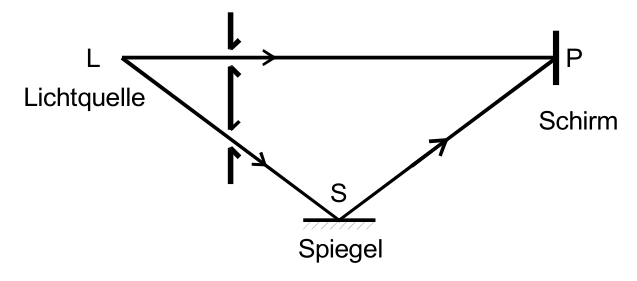
\includegraphics[width=0.8\textwidth]{latex/images/konvenL.PNG}
            \caption{Prinzipielle Versuchsordnung zur Erzeugung von Interferenzerscheinung unter Verwendung einer konventionellen 
            Lichtquelle \protect \cite{V401}.}
            \label{img:konv}
        \end{figure}

        \noindent Im folgenden wird die Kohärenzlänge $l$ und die Verteilung $\Delta \omega$ der Frequenzverteilung untersucht, 
        dazu wird ein sinusförmiger Wellenzug endlicher Länge

        \begin{equation*}
            E(t) = E_0 \text{e}^{-i \omega_0 t} \quad \quad \text{für} -\frac{\tau}{2} < t < \frac{\tau}{2} \nonumber
        \end{equation*}

        \noindent weiter angeschaut. Die Fouriertransformation dieser Welle ergibt

        \begin{equation}
            g(\omega) = E_0 \int_{-\tau / 2}^{-\tau /2} \text{e}^{i(\omega - \omega_0)} \text{d}t = E_0 
            \frac{\text{sin}(\omega - \omega_0) \tau}{\omega - \omega_0} \nonumber
        \end{equation}

        \noindent und somit die Intensität

        \begin{equation*}
            I = G(\omega) = |g(\omega)|^2 = E_0^2 
            \frac{\text{sin}^2(\omega - \omega_0) \tau^2}{(\omega - \omega_0)^2} \nonumber
        \end{equation*}

        \noindent Aus diesem Ausdruck ist nun ein Maximum bei $\omega = \omega_0$ und ein Minimum bei
    
        \begin{equation}
            \omega_{\text{N}} = \omega_0 \pm 2\frac{\pi}{\tau}          \nonumber     
        \end{equation}

        \noindent abzulesen. Weiterhin ist zu erkennen, dass der größter Teil der Energie im Bereich 

        \begin{equation}
            \omega_0 - 2\frac{\pi}{\tau} < \omega < \omega_0 + 2\frac{\pi}{\tau}    \nonumber 
        \end{equation}

        \noindent liegt. Dieser Bereich bzw. diese Breite ist die Verteilungsfunktion 

        \begin{equation}
            \Delta \omega = 2 \frac{\pi}{\tau}
            \label{eqn:1}
        \end{equation}

        \noindent Die Breite der Wellenlängenverteilung kann durch die Formel 

        \begin{equation}
            \lambda_0 := \frac{2 \pi \text{c}}{\omega_0}    \nonumber 
        \end{equation}

        \noindent ausgedrückt werden. Differentieren und einstzten von Formel (\ref{eqn:1}) ergibt dann 

        \begin{equation}
            \Delta \lambda = \frac{\lambda_0^2}{\text{c}\tau},     \nonumber 
        \end{equation}

        \noindent über die Kohärenzzeit $\tau = \frac{l}{c}$ ergibt sich 

        \begin{equation}
            \Delta \lambda = \frac{\lambda_0^2}{l}.    \nonumber 
        \end{equation}

        \noindent Auch die Polarisation muss noch kurz betrachtet werden, denn falls das Licht polarisiert ist, entsteht nur Interferenz 
        wenn die Lichtquellen nicht senkrecht zueinander polarisiert sind da sonst das Skalarprodukt 
     
        \begin{equation}
            \vec{\text{E}}_1 \cdot \vec{\text{E}}_2     \nonumber 
        \end{equation}

        \noindent gleich 0 ist.

    \subsection{Fourier-Spektroskopie mit dem Michelson-Interferometer}

            \noindent Wird die gemessene Lichtintensität in Abhängigkeit von der Spiegelverschiebung $L(x)$ fouriertransformiert ist es möglich 
            die spektrale Verteilung der Lichtquelle zu bestimmen. Nach den Fourierschen Theorem gilt 

            \begin{equation*}
                 \text{G}(k) = \frac{1}{2\pi} \int_{- \infty}^{\infty} L(x) \text{e}^{ikx} \text{d}x    \nonumber 
            \end{equation*}

            \noindent mit der Wellenzahl $k$ und der zugehörigen Intensität G$(k)$. Es wird also eine möglichst große Spiegelverschiebung gemessen 
            und dann die Fouriertransformation numerisch berechnet. Das einzige Limit dieser Methode ist die Messgenauigkeit des Interferometers und 
            die Rechenleistung des Computers.

    \subsection{Prinzipieller Aufbau des Michelson Interferometers-Interferometers }

        \noindent Generells sind Interferometer Geräte die mittels interferenzeffekten optische Größen messen. Im Michelson Interferometer wird 
        Interferenz dadurch ermöglicht, dass ein Strahl in mindestens zwei Teilbündel aufgeteilt wird und wieder zusammen geführt wird nach  
        dem einer der Teilstrahlen verädert wird. Die Aufteilung geschieht hier wie in Abbildung(\ref{img:4}) zu sehen ist, 
        durch eine semipermeable Platte.

        \begin{figure}[ht]
            \centering
            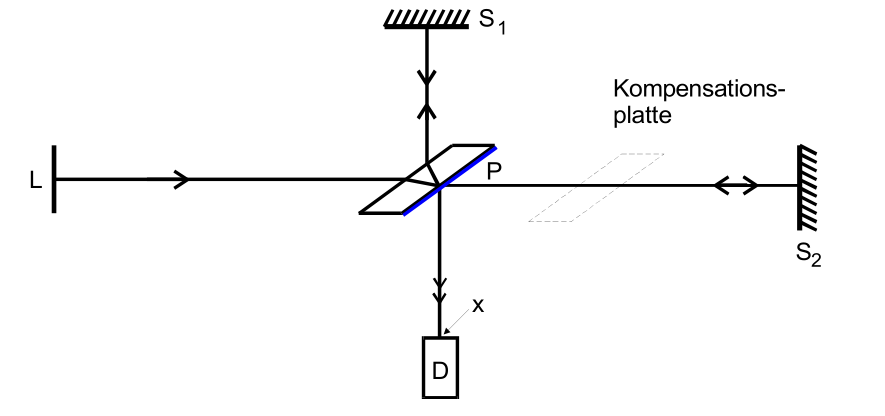
\includegraphics[width=0.7\textwidth]{latex/images/PrinAuf.PNG}
            \caption{Schematischer AUfbau des Michelson-Interferometers (L = Lichtquelle, S$_1$ und S$_2$ Spiegel, P = semipermeabler Spiegel, 
            D = Lichtdetektor)\protect \cite{V401}.}
            \label{img:4}
        \end{figure}

        \noindent Die Teilbündel werden denn an den Spiegel S$_1$ und S$_2$ wieder auf die semipermeable Platte P reflektiert. Von dort werden dann 
        Teile des Lichts auf den Lichtdetektor geleitet, falls der Wegunterschied nicht größer als die Köhärenzlänge ist, sind die 
        beiden Lichtstrahlen auch kohärent. Um das zu ermöglichen wird auf der Seite des S$_2$ Spiegels eine Kompensationsplatte in den 
        Weg des Lichtstrahls gestellt um die Diskrepanz an der semipermeablen Platten auszugleichen. Ist nun also $\overline{\symup{S_1P}}$ 
        gleich $\overline{\symup{S_2P}}$ entsteht eine destruktive Interferenz aufgrund des $\lambda / 2$ Wegunterschied des Phasensprungs 
        an dem P Spiegel bei der zweiten Reflektion. Wird jetzt eber ein Spiegel um die Länge $d$ verschoben, entsteht zwischen den beiden 
        Lichtstrahlen ein Wegunterschied von $w = 2d$, dadurch ändert sich das Interferenzverhalten. Diese Verschiebung lässt sich mit den 
        Formeln der elektrischen Feldstärke der einzelnen Wellen beschreiben. Diese sind

        \begin{equation}
            \vec{E}_1(x) = \vec{E}_0 \text{e}^{ikx} \quad \quad \text{und} \quad \quad \vec{E}_2(x) = \vec{E}_0 \text{e}^{ikx + 2d +\pi} ,    \nonumber 
        \end{equation}

        \noindent und mit 

        \begin{equation*}
            k = \frac{2 \pi}{\lambda}
        \end{equation*}

        \noindent folgt

        \begin{align}
            I(d) &= \vec{E}_0^2 \left( \text{e}^{ikx} + \text{e}^{ik(x + 2d + \pi)} \right) \left( \text{e}^{-ikx} + \text{e}^{-ik(x + 2d + \pi)} \right) \\    \nonumber 
                 &= 2 \cdot \vec{E}_0^2  \left( 1 + \text{cos} \left( \frac{2 \pi}{\lambda} 2 d + \pi \right) \right)    \nonumber 
        \end{align}

        \noindent Somit schwankt $I(d)$ periodisch zwischen 0 und einem Maximum wenn d verändert wird. Es lässt sich also hiermit mittels der 
        Verschiebung $\Delta d$ und der Anzahl der Maxima $z$ über 

        \begin{equation}
            \Delta d = z \cdot \frac{\lambda}{2}    \nonumber 
        \end{equation}

        \noindent die Wellenlänge bestimmen.\\

        Des weiteren lässt sich innerhalb des Interferometers ein Weglängenunterschied generieren in dem ein Medium mit einem anderen 
        Brechungsindex in den Strahlengang geführt wird, skizziert ist dies in Abbildung(\ref{img:5}).

        \begin{figure}[ht]
            \centering
            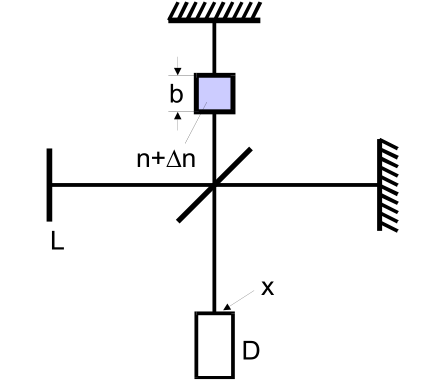
\includegraphics[width=0.4\textwidth]{latex/images/PrinOrd.PNG}
            \caption{Prinzipieller Versuchsaufbau zur Messung von Brechungsindeces mit Hilfe des Michelson-Interferometers \protect \cite{V401}.}
            \label{img:5}
        \end{figure}

        \noindent Nun durchläuft das Licht ein Medium mit dem Brechungsindex $n+\Delta n $ und der Breite $b$, wir $b$ ausgedehnt, laufen 
        dann nach der Formel

        \begin{equation}
            b \cdot \Delta n = \frac{z \lambda}{2}    \nonumber 
        \end{equation}

        \noindent $z$ Maxima über den Sensor. Weiterhin gilt nach der klassischen Dispersionstheorie, dass sich der Brechungsindex nach 
        
        \begin{equation}
            n = \sqrt{1 + f(\lambda) N}    \nonumber 
        \end{equation}

        \noindent aus der Anzahl der Dipole pro Volumeneinheit die durch die Wellenlänge angeregt werden, berechnen lässt. Die hier benutzten 
        Gase werden durch die Ideale Gasgleichung 
        
        \begin{equation}
            N(r,T) = \frac{p}{T} \frac{T_0}{p_0} N_{\text{L}}    \nonumber 
        \end{equation}

        \noindent beschreiben, da im Bereich von 0 bis 1 Bar gemessen wird. Die Differenz berechnet sich somit nach 
        $\Delta n(p,p') = \frac{f}{2}(N(p,T)-N(p',T))$ und unter Normalbedingungen ist 

        \begin{equation}
            n(p_0, T_0) = 1 + \Delta n(p,p') \frac{T}{T_0} \frac{p_0}{p-p'}.    \nonumber 
        \end{equation}

        \noindent Hiermit kann nun der Brechungsindex mittels 

        \begin{equation}
            n = 1 + z \cdot \frac{\lambda}{2b} \cdot \frac{T}{T_0} \frac{p_0}{p - p'}    \nonumber 
        \end{equation}

        \noindent berechnet werden.